One severe issue for current chit-chat systems is their lack of speaker consistency. 
Since the training set contains conversations from different people, and a decoding model always selects the response with the greatest likelihood,
outputs can be wildly inconsistent, as illustrated in Table \ref{sample:baseline}. 
\begin{table}
\center
\begin{tabular}{rlrl}\toprule
m: & Where do you live now?&m:  & Where were you born?\\
r: & I live in Los Angeles.&r: & I was born in Canada.  \\
m:  & In which city do you live now?& m:  & Where are you from?\\
r: & I live in Madrid.& r: & England, you?\\
m:  & In which country do you live now?&m:  & Where did you grow up?\\
r: & England, you?& r: & I grew up in Texas.\\\midrule
m:  & How old are you?&m:  & What is your major? \\
r: & 16 and you?& r:&I'm majoring in psychology \\
m:  & What's your age?&m:  & What did you study in college?\\
r: & 16. &r:& I studied psychology. \\\bottomrule
\end{tabular}
\caption[Inconsistent responses from \sts models]{Inconsistent responses generated by a 4-layer \sts model trained on 25 million Twitter conversation snippets. m denotes input message and r denotes the generated response.}
\label{sample:baseline}
\end{table}

In this chapter, we 
talk about how we can 
address the challenge of consistency and how to endow data-driven systems with the coherent ``persona'' needed to model human-like behavior, whether as personal assistants, personalized avatar-like agents, or game characters.\footnote{\newcite{vinyals2015neural} suggest that the lack of a coherent personality makes it impossible for current systems to pass the Turing test.} 
For present purposes, we will define \textsc{persona} as the character that an artificial agent, as actor, plays or performs during conversational interactions.
A~persona can be viewed as a composite of elements of identity (background facts or user profile), language behavior, and interaction style. 
A persona is also adaptive, since an agent may need to present different facets to different human interlocutors depending on the demands of the interaction. 


We explore two persona models, a single-speaker \textsc{Speaker Model} and a dyadic \textsc{Speaker-Addressee Model}, within the \sts framework. 
The Speaker Model integrates a speaker-level vector representation into the target part of the \sts model.
Analogously, the Speaker-Addressee model encodes the interaction patterns of two interlocutors by constructing an interaction representation from their individual embeddings and incorporating it into the \sts model. 
These persona vectors are trained on human-human conversation data and used at test time to generate personalized responses.
Our experiments on an open-domain corpus of Twitter conversations and dialog datasets comprising TV series scripts show that leveraging persona vectors can improve relative performance up to $20\%$ in \bleu score and $12\%$ in perplexity, with a commensurate gain in consistency as judged by human annotators. 





\begin{figure*} [!ht]
%\begin{figure*}
\centering
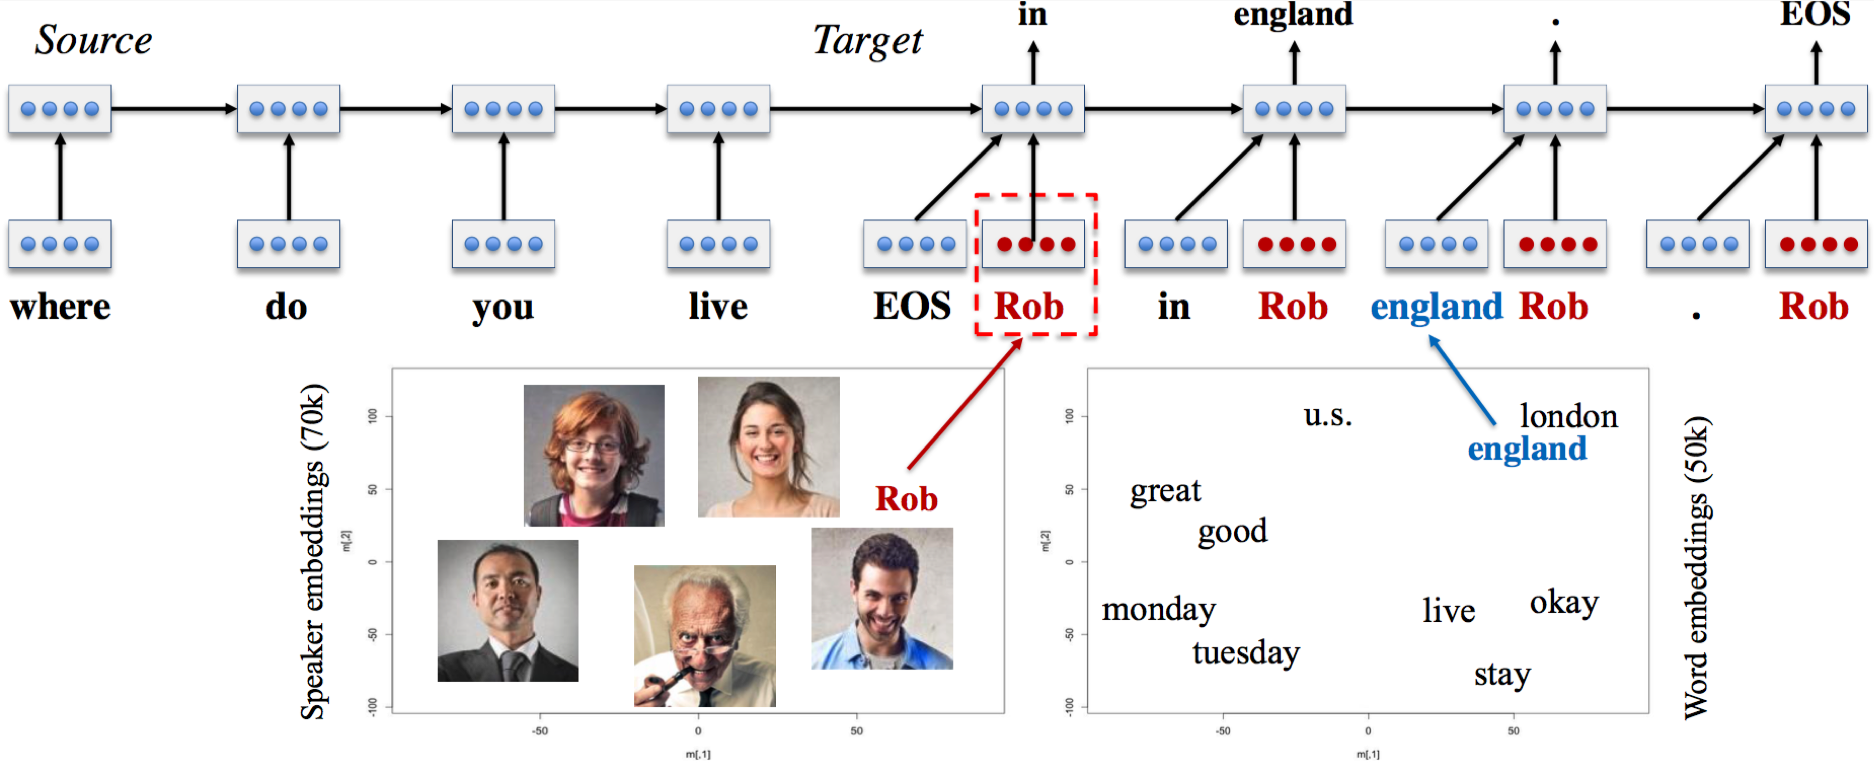
\includegraphics[width=6in]{img/persona.png}
%\includegraphics[width=5.2in]{1.png}
\caption[The persona speaker model]{Illustrative example of the Speaker Model introduced in this work. Speaker IDs close in embedding space tend to respond in the same manner. These speaker embeddins are learned jointly with word embeddings and all other parameters of the neural model via backpropagation. % through time. % (BPTT).
In this example, say Rob is a speaker clustered with people who often mention England in the training data, then the generation of the token `england' at time \mbox{$t=2$} would be much more likely than that of `u.s.'. A non-persona model would prefer generating {\it in the u.s.} if `u.s.' is more represented in the training data across all speakers.
}\label{fig1}
\end{figure*}

\section{Model}
\subsection{Speaker Model}
Our first model is the Speaker Model, which 
models the respondent alone.
This model represents each individual speaker as a vector or embedding, which encodes 
speaker-specific information (e.g., dialect, register, age, gender, personal information) that influences the content and style of her responses.\footnote{Note that these attributes are not explicitly annotated, which would be tremendously expensive for our datasets. Instead, our model manages to cluster users along some of these traits (e.g., age, country of residence) based on responses alone.}
%the speaker says, such as gender, age, speaking style, and any person-specific %information that influences what the speaker  %says.
%% MG to Jiwei: what does this mean?
%%User representations will then be incorporated into neural models at decoding time. 

Figure \ref{fig1} gives a brief illustration of the Speaker Model. 
Each speaker $i\in [1,N]$ is associated with a user-level representation $v_i\in\mathbb{R}^{K\times 1}$. 
 As in standard \sts models, we first encode message  $S$ into a vector representation $h_S$ using the source LSTM. 
Then for each step in the target side, hidden units are obtained by 
combining the representation produced by the target LSTM at the previous time step (i.e., $h_{t-1}$), the word representations at the current time step $x_t$, and the speaker embedding $v_i$:
\begin{equation}
\left[
\begin{array}{lr}
i_t\\
f_t\\
o_t\\
l_t\\
\end{array}
\right]=
\left[
\begin{array}{c}
\sigma\\
\sigma\\
\sigma\\
\tanh\\
\end{array}
\right]
W\cdot
\left[
\begin{array}{c}
v_i\\
h_{t-1}\\
x_t\\
\end{array}
\right]
\end{equation}
\begin{equation}
c_t=f_t\cdot c_{t-1}+i_t\cdot l_t
\end{equation}
\begin{equation}
h_{t}=o_t\cdot \tanh(c_t)
\end{equation}
where $W\in \mathbb{R}^{4K\times 3K}$. 
In this way, speaker information is encoded and 
injected into the hidden layer at each time step and thus helps predict personalized responses throughout the generation process.
%In this way, speaker information is encoded and then incorporated to each step of word predicting to guide decoding process. 
The Speaker embedding $\{v_i\}$ is shared across all conversations that involve speaker $i$.  $\{v_i\}$ are learned by back propagating word prediction errors to each neural component during training. 

Another helpful property of this model is that it 
helps {\it infer} answers to questions even if the evidence is not readily present in the training set.
This is important as
%Another helpful property of this model is that it allows for inference about the answers to the input questions even if the evidence is not readily present in the training set.  
the training data does not contain explicit 
%evidence about concrete facts for every 
information about every
attribute of each user
(e.g., gender, age, country of residence).

The model learns speaker representations based on conversational content produced by different speakers, and speakers producing similar responses tend to have similar embeddings, occupying nearby positions in the vector space. 
This way, the training data of speakers nearby in vector space help increase the generalization capability of the
speaker model. For example, consider two speakers $i$ and $j$
who sound distinctly British, and who are therefore close in speaker 
embedding space. Now, suppose that, in the training data, speaker $i$ was asked {\it Where do you live?} and responded {\it in the UK}. Even if speaker $j$ was never asked the same question, this answer can help influence a good response from speaker $j$, and this without any explicitly labeled geo-location information.
  
\subsection{Speaker-Addressee Model}
%One step further over speaker model is to model speaker-speaker interacting patterns within the conversation as
A natural extension of the Speaker Model is a model that is sensitive to speaker-addressee interaction patterns within the conversation. Indeed,
speaking style, register, and content does not only vary with the identity of the speaker, but also with that of the addressee.
For example, in scripts for the TV series {\it Friends} used in some of our experiments, the character Ross often 
talks differently to his sister Monica than to Rachel,
with whom he is engaged in a on-again off-again relationship throughout the series. 

The proposed Speaker-Addressee Model operates as follows:
We wish to predict how speaker $i$ would respond to a message produced by speaker $j$. Similarly to the Speaker model, we associate each speaker with a $K$ dimensional speaker-level representation, namely $v_i$ for user $i$ and $v_j$ for user $j$. 
We obtain an interactive representation $V_{i,j}\in \mathbb{R}^{K\times 1}$ by linearly combining user vectors $v_i$ and $v_j$
in an attempt to model the interactive style of user $i$ towards user $j$,
\begin{equation}
V_{i,j}=\tanh(W_1\cdot v_i+W_2\cdot v_2)
%\label{equ9}
\end{equation}
where $W_1, W_2\in \mathbb{R}^{K\times K}$. 
$V_{i,j}$  is then linearly incorporated into LSTM models at each step in the target: 
\begin{equation}
\left[
\begin{array}{lr}
i_t\\
f_t\\
o_t\\
l_t\\
\end{array}
\right]=
\left[
\begin{array}{c}
\sigma\\
\sigma\\
\sigma\\
\tanh\\
\end{array}
\right]
W\cdot
\left[
\begin{array}{c}
h_{t-1}\\
w_{t}\\
V_{i,j}\\
\end{array}
\right]
\end{equation}
\begin{equation}
c_t=f_t\cdot c_{t-1}+i_t\cdot l_t\\
\end{equation}
\begin{equation}
h_{t}=o_t\cdot \tanh(c_t)
%h_{t}^s=o_t\cdot \text{tanh}(f_t\cdot c_{t-1}+i_t\cdot l_t)
\end{equation}
$V_{i,j}$ 
%is obtained based on current speaker and the speaker he is talking too. 
depends on both speaker and addressee and
the same speaker will thus respond differently to a message from different interlocutors. 
%Such a mechanism allows us the model the interaction styles between different speakers. 
One potential issue with Speaker-Addressee modelling is the difficulty involved in collecting a large-scale training dataset in which each speaker 
is involved in conversation with a wide variety of people. Like the Speaker Model, however, the Speaker-Addressee Model derives generalization capabilities from speaker embeddings.
Even if the two speakers
at test time ($i$ and $j$) were never involved in the same conversation in the training data, two speakers $i'$ and $j'$ who are respectively close in embeddings may have been, and this can help  modelling how $i$ should respond to $j$. 

\subsection{Decoding and Reranking}
For decoding, 
the N-best lists  are generated using the decoder with beam size \mbox{$K=200$}.
We set a maximum length of 20 for the generated candidates. 
To deal with the issue that \sts models tend to generate generic and commonplace responses such as {\it I don't know}, we follow \newcite{li2015diversity} by reranking the generated N-best list 
using a scoring function that linearly combines 
 a length penalty and the log likelihood of source given target:
\begin{equation}
%Score(R)=\\
\log p(y|x,v)+\lambda\log p(x|y)+\gamma L_y 
\end{equation}
where $p(y|x,v)$ denotes the probability of the generated response given the message $x$ and the  respondent's speaker ID. 
$L_y$ denotes the length of the target and $\gamma$ denotes the associated penalty weight. We optimize $\gamma$ and $\lambda$ on N-best lists of response candidates generated from the development set using MERT \cite{och2003minimum} by optimizing \bleu.
To compute $p(x|y)$, 
we train an inverse \sts model by swapping messages and responses. We trained standard \sts models for $p(x|y)$  with no speaker information considered.  



\section{Experiements}
Following \cite{sordoni2015neural,li2015diversity}
we used \bleu \cite{papineni2002bleu} 
for parameter tuning and evaluation. 
Besides \bleu scores, we also report perplexity, which has been widely adopted as an indicator of model capability. 

\begin{table}
\centering
\begin{tabular}{lc}\toprule
System                                    & \bleu \\ \midrule
MT baseline \cite{ritter2011data}         & 3.60\% \\ 
Standard LSTM MMI \cite{li2015diversity}  & 5.26\% \\
Standard LSTM MMI (our system)            & 5.82\% \\ 
{\it Human}                               & {\it 6.08\%}\\\bottomrule
\end{tabular}
\caption[Results for the baseline model]{\bleu on the Twitter Sordoni dataset (10 references). We contrast our baseline against an SMT baseline \cite{ritter2011data}, and the best result \cite{li2015diversity} on the established
dataset of \cite{sordoni2015neural}.
The last result is for a human oracle, but it is not directly comparable as the oracle \bleu is computed in a leave-one-out fashion, having one less reference available. We nevertheless provide
this result to give a sense that these \bleu scores of 5-6\% are not unreasonable.}
\label{twitter-baselines}
\end{table}

\subsection{Baseline}
Since our main experiments are with a new dataset (the Twitter Persona Dataset), we first show that our LSTM baseline is competitive with the state-of-the-art \cite{li2015diversity} on an established
dataset, the Twitter  Dataset \cite{sordoni2015neural}.
Our baseline is simply our implementation of the LSTM-MMI of \cite{li2015diversity}, so results should be relatively close to their reported results.
Table~\ref{twitter-baselines} summarizes our results against prior work.
We see that our system actually does better than \cite{li2015diversity}, and
we attribute the improvement to a larger training corpus, the use of dropout during training, and possibly to the ``conversationalist'' nature of our corpus.

%In this section, we present quantitative evaluation results of the %proposed model on the two datasets, along with qualitative analysis. 
\begin{table}
\centering
\begin{tabular}{ccc}\toprule
Model&Standard LSTM&Speaker Model \\\midrule
Perplexity&47.2&42.2 ($-10.6\%$) \\\bottomrule
\end{tabular}
\caption[Perplexity for the persona model on the Twitter dataset]{Perplexity for standard \sts and the Speaker model on the development set of the Twitter Persona dataset.}
\label{twitter-per}
\end{table}
\begin{table}
\centering
\begin{tabular}{lll}\toprule
Model&Objective& \bleu \\\midrule
Standard LSTM &MLE& 0.92\% \\
Speaker Model & MLE&1.12\%  \\
Standard LSTM &MMI& 1.41\% \\
Speaker Model & MMI&1.66\%\\\bottomrule
\end{tabular}
\caption[\bleu for the persona model on the Twitter dataset]{
\bleu on the Twitter Persona dataset (1 reference), for the
standard \sts model and the Speaker model using as objective either maximum likelihood (MLE) or maximum mutual information (MMI).}
\label{twitter-bleu}
\end{table}

\begin{table*}
\centering
\begin{tabular}{cccc}\toprule
Model&Standard LSTM&Speaker Model& Speaker-Addressee Model \\
Perplexity&27.3&25.4 ($-7.0\%$)& 25.0 ($-8.4\%$)  \\\bottomrule
\end{tabular}
\caption[Perplexity for the persona model on the TV series dataset]{Perplexity for standard \sts and persona models on the TV series dataset.}
\label{tv-per}
\end{table*}
\begin{table*}
\centering
\begin{tabular}{ccccc}\toprule
Model&Standard LSTM&Speaker Model& Speaker-Addressee Model \\\midrule
MLE&1.60\%& 1.82\% ($+13.7\%$)& 1.83\%  ($+14.3\%$) \\
MMI&1.70\%& 1.90\% ($+10.6\%$) &1.88\% ($+10.9\%$) \\\bottomrule
\end{tabular}
\caption[\bleu for the persona model on the TV series dataset]{
\bleu on the TV series dataset (1 reference), for the
standard \sts and persona models.}
\label{tv-bleu}
\end{table*}

\subsection{Results}
We first report performance on the Twitter Persona dataset.
%in Table~\ref{twitter-per}. The baseline is the standard \sts model with both standard likelihood objective and mutual information reranking using beam size 200. 
Perplexity is reported in Table \ref{twitter-per}. We observe about a $10\%$ decrease in perplexity for the Speaker model over the standard \sts model. 
In terms of \bleu scores (Table~\ref{twitter-bleu}), a significant performance boost 
is observed for 
 the Speaker model over the standard \sts model, yielding an increase of $21\%$
in the maximum likelihood (MLE) setting and $11.7\%$ for mutual information setting (MMI). 
In line with findings in \cite{li2015diversity}, we observe a consistent performance boost introduced by 
the MMI objective function 
over a standard \sts model based on the MLE objective function. 
It is worth noting that our persona models are more beneficial to the MLE models
than to the MMI models. This result is intuitive as the persona models help make 
Standard LSTM MLE outputs more informative and less bland, and thus make the use 
of MMI less critical.


For the TV Series dataset,  perplexity and \bleu  scores are respectively  reported in Table \ref{tv-per} and Table \ref{tv-bleu}.
As can be seen, the Speaker and Speaker-Addressee models respectively achieve perplexity values of 25.4 and 25.0 on the TV-series dataset, $7.0\%$ and $8.4\%$ percent lower than the correspondent standard \sts models. 
In terms of \bleu score,  we observe a similar performance  boost as on the Twitter dataset, in which the Speaker model
and the Speaker-Addressee model 
 outperform the standard \sts model by $13.7\%$ and $10.6\%$.
By comparing the Speaker-Addressee model against the Speaker model on the TV Series dataset, we do not observe a significant difference.  
We suspect that this is primarily due to the relatively small size of the dataset where the interactive patterns might not be fully captured. 
Smaller values of perplexity are observed for the Television Series dataset than the Twitter dataset, the perplexity of which is over 40, presumably due to the more noisy nature of Twitter dialogues. 
\subsection{Qualitative Analysis}

\begin{table}
\setlength{\tabcolsep}{4pt}
\center
{\small
\begin{tabular}{rlrl} \toprule
\Message   & Where is your hometown?&\Message   & What company do you work for? \\\midrule
{\it baseline}    & I was born in Canada.&{\it baseline}    & I work for a company.\\\midrule
\User{1}   & I'm from England.&\User{1}   & I don't have a job.\\
\User{2}   & I'm from Manchester.& \User{2}   & I'm a manager.\\
\User{3}   & I'm from Liverpool.&\User{3}   & I'm working. {\color{red} $\#$}\\
\User{4}   & England. You?&\User{4}   & I work for a company\\
\User{5}   & My hometown.&\User{5}   & I'm working. {\color{red} $\#$}\\
\User{6}   & I'm from Texas.&\User{6}   & Customer service.\\
\User{7}   & I'm from LA.&\User{7}   & I work in retail.\\
\User{8}   & England.&\User{8}   & I work in a cafe.\\
\User{9}   & I was born here.&\User{9}   & I work at a gas station.\\
\User{10}  & I was born in the us.&\User{10}  & I don't know {\color{red} $\#$}\\\bottomrule
\end{tabular}
}
\caption[Sample responses from the persona model on the Twitter dataset]{Responses generated by the baseline (LSTM-MMI) and the Speaker Model for ten randomly selected users, without cherry picking. {\color{red} $\#$} indicates poor-quality responses produced by the system.}
\label{example1}
\end{table}


\begin{table}[!ht]
\setlength{\tabcolsep}{4pt}
\center
{\small
\begin{tabular}{cc} \toprule
\Message   & Do you love me ?\\\midrule
{\it baseline} & of course, i love you .  \\\midrule
& {\it addressee {\it Emily},  speaker Sheldon }\\
{\it response} & of course, i love you, emily .\\\midrule
& {\it addressee {\it Emily},  speaker Penny }\\
{\it response} & of course, i love you, emily .\\\midrule
& {\it addressee {\it Lenard},  speaker Penny }\\
{\it response} & of course, i love you, Lenard .\\\midrule
& {\it addressee {\it Monica},  speaker  Chandler }\\
{\it response} & of course i love you . i want to marry you .\\\midrule
& {\it addressee {\it  Rachel},  speaker  Chandler }\\
{\it response} & of course i love you .\\\midrule
& {\it addressee {\it  Ross},  speaker  Chandler }\\
{\it response} & of course i love you .\\\midrule
& {\it addressee {\it  Ross},  speaker  Rachel }\\
{\it response}  &of course i love you . ( kisses him ) \\\midrule
& {\it addressee {\it  Emily},  speaker  Rachel }\\
{\it response}  &of course i love you . \\\bottomrule
\end{tabular}
}
\caption[Sample responses from the addressee-speaker model on the TV-series dataset]{Responses to {\it do you love me} from the {\it addressee-speaker} model on the TV-series dataset using different addressees and speakers.}
\label{addressees}
\end{table}



\paragraph{Diverse Responses by Different Speakers}
Table \ref{example1} represents responses generated by persona models in response to three different input questions. We randomly selected 10 speakers (without cherry-picking) from the original Twitter dataset. We collected their user level representations from a speaker look-up table and integrated them into the decoding models.  We can see that the model tends to generate specific responses for different people in response to the factual questions.\footnote{There appears to be a population bias in the training set that favors British users.}  

Table \ref{addressees} represents responses generated from the {\it Speaker-Addressee Model} using the TV-series dataset. Interestingly, we do observe the subtle difference captured by the model when it 
attempts to respond to different 
addresses . For example, the model produces {\it of course, i love you, emily .} in response to input from addressee{\it Emily} by generating the addressee's name. 
Also, the model generates {\it of course i love you . ( kisses him )} in response to female addressees. 
 
% that there's a bias for some answers than others. For example, British locations tend to appear more often than others, and also British food such as {\it fish and chips}. This might be caused by the 
\paragraph{Human Evaluation} We conducted a human evaluation of outputs from the Speaker Model, using 
a crowdsourcing service. 
%an in-house crowdsourcing service. 
Since we cannot expect crowdsourced human judges to know or attempt to learn the ground truth of Twitter users who are not well-known public figures, we designed our experiment to evaluate the consistency of outputs associated with the speaker IDs. To this end, we collected 24 pairs of questions for which we would expect responses to be consistent if the persona model is coherent.  For example, responses to the questions {\it What country do you live in?} and {\it What city do you live in?} would be considered consistent if the answers were {\it England} and {\it London} respectively, but not if they were {\it UK} and {\it Chicago}.  Similarly, the responses to {\it Are you vegan or vegetarian?} and {\it Do you eat beef?} are consistent if the answers generated are {\it vegan} and {\it absolutely not}, but not if they are {\it vegan} and {\it I love beef}.  We collected the top 20 pairs of outputs provided by the Speaker Model for each question pair (480 response pairs total). We also obtained the corresponding outputs from the baseline MMI-enhanced \sts system. 

Since our purpose is to measure the gain in consistency over the baseline system, we presented the pairs of answers system-pairwise, i.e., 4 responses, 2 from each system,  displayed on the screen.
Then we 
 asked judges to decide which of the two systems was more consistent.  The position in which the system pairs were presented on the screen was randomized.  Five judges rated each pair.  A system was assigned a score 1.0 if it was judged much more consistent than the other, 0.5 if mostly more consistent, zero otherwise. Ties (where the two systems are equally consistent or inconsistent) were discarded.  A maximum score of 5.0 was possible. After reweighting for frequency of response  pairs, the mean relative consistency rating for the Speaker Model was 1.33 compared to 0.99 for the baseline model, representing a gain in relative consistency of 34.68\%. It should be stressed that the latter is a strong baseline, since it represents the consensus of all 70K Twitter users in the dataset. ({\it I'm not pregnant} is an excellent consensus answer to the question {\it Are you pregnant?}, while {\it I'm pregnant} is consistent as a response only in the case of someone who also answers the question {\it Are you a guy or a girl?} with something in the vein of {\it I'm a girl}.)

\paragraph{Speaker Consistency}
Table \ref{example2} illustrates how consistency is an emergent property of two arbitrarily selected users. The model is capable of discovering the relations between different categories of location such as London and the UK, Jakarta and Indonesia. However, the model also makes inconsistent response decisions, generating different answers in the second example in response to questions asking about age or major. 
Our proposed persona models integrate user embeddings into the LSTM, and thus can be viewed as encapsulating a trade-off between a persona-specific generation model and a general conversational model. 



\begin{table}[!ht]
\setlength{\tabcolsep}{4pt}
\center
{\small
\begin{tabular}{rlrl} \toprule
{\bf User1} &&{\bf User2}&\\\midrule
\Message    & Where is your hometown?&\Message    & Where is your hometown?\\
\Response   & I'm from England.& \Response   & I live in Indonesia.\\\
\Message    & Where are you from?&\Message    & Where are you from? \\
\Response   & I'm from England.&\Response   & England, you? \\
\Message    & In which city do you live now?&\Message    & In which city do you live now?\\
\Response   & I live in London.& \Response   & I live in Jakarta.\\
\Message    & In which country do you live now?&\Message& In which country do you live now? \\
\Response   & I live in England.&\Response   & I live in Indonesia. \\\midrule
\Message    & What is your major?&\Message    & What is your major?\\
\Response   & Business. You?& \Response   & Business, you?\\
\Message    & What did you study in college?&\Message    & What did you study in college?\\
\Response   & I did business studies.& \Response   & Psychology, you?\\\midrule
\Message    & How old are you?&\Message    & How old are you? \\
\Response   & I'm 18.&\Response   & I'm 18.\\
\Message    & What is your age?&\Response& What is your age?\\
\Response   & I'm 18. &\Response&  I'm 16.\\\bottomrule
\end{tabular}
}
\caption{Examples of speaker consistency and inconsistency generated by the Speaker Model}
\label{example2}
\end{table}
\section{Conclusion}
In this chapter,
we have presented two persona-based response generation models for open-domain conversation generation. 

Although the gains presented by our new models are not spectacular, the systems nevertheless outperform our baseline \sts systems in terms of \bleu, perplexity, and human judgments of speaker consistency. 
We have demonstrated that by encoding personas into distributed representations, we are able
to capture certain personal characteristics such as speaking style and background information. 
In the Speaker-Addressee model, moreover, the evidence suggests that there is benefit in capturing dyadic interactions. 

Our ultimate goal is to be able to take the profile of an arbitrary individual whose identity is not known in advance, and generate conversations that accurately emulate that individual's persona in terms of linguistic response behavior and other salient characteristics. 
Such a capability will dramatically change the ways in which we interact with dialog agents of all kinds, opening up rich new possibilities for user interfaces. 
Given a sufficiently large training corpus in which a sufficiently rich variety of speakers is represented, this objective does not seem too far-fetched.




%We conducted experiments on both the open-domain dialogue corpus from Twitter and domain-specific dataset using scripts from TV series. 
%We observe that leveraging personal information bring out significant performance boost at qualitative level up to $20\%$ in term of BLEU score and $12\%$ in terms of perplexity. 
%Qualitative analysis demonstrates that the model has the capability of handling speaker-consistency %issue in dialogue generation.

%The rest of this paper is organized as follow: Section 2 describes related work. Section 3 details \sts models that we use.
%Section 4 details the proposed algorithms for speaker modeling. Section 5 presents dataset we use. 
%Experimental results are presented in Section 6 followed by a brief conclusion. 
